\documentclass[a4paper,landscape]{standalone}
\usepackage[utf8]{inputenc}
\usepackage{tikz}
\usetikzlibrary{positioning}
\title{Project Canvas}

% Colours
\definecolor{top}{RGB}{105,105,105}
\definecolor{bottom}{RGB}{245,245,220}
\definecolor{second}{RGB}{22,250,150}
\definecolor{risk}{RGB}{251,229,214}

% Styles
\tikzstyle{smallblock} = [execute at begin node=\setlength{\baselineskip}{2.5em}, text width=38em, node distance=.5em, minimum width= 40em, minimum height=10em, text depth=8em, text height=2.5em]
\tikzstyle{block} = [execute at begin node=\setlength{\baselineskip}{2.5em}, text width=38em, node distance=.5em, minimum width= 40em, minimum height=14em, text depth=12em, text height=2.5em]
\tikzstyle{bigblock} = [execute at begin node=\setlength{\baselineskip}{2.5em}, text width=38em, node distance=.5em, minimum width= 40em, minimum height=20em, text depth=17em, text height=2.5em]
\tikzstyle{megablock} = [execute at begin node=\setlength{\baselineskip}{3em}, text width=78em, node distance=.5em, minimum width= 80.5em, minimum height=34.5em, text depth=32.25em,text height=3em]

% Definitions
\newcommand\client[2]{\node[smallblock,fill=top,text=white,] (client) {\raggedright\Huge \textbf{Professor/Disciplina:}\\[1em]\huge #1 \\\normalsize #2};}

\newcommand\project[1]{\node[smallblock,right= of client,fill=top,text=white,] (project) {\raggedright\Huge \textbf{Título do projeto:} \normalsize \\[1em]\huge #1};}

\newcommand\manager[1]{\node[smallblock,right= of project,fill=top,text=white,] (manager) {\raggedright\Huge \textbf{Componentes do grupo:} \normalsize \\[1em]\huge #1};}

\newcommand\why[1]{\node[block,below= of client,fill=second] (why) {\raggedright\Huge \textbf{Objetivo:} \normalsize \\[1em]\huge #1};}

\newcommand\what[1]{\node[block,right= of why,fill=second] (what) {\raggedright\Huge \textbf{Contexto:}\\[1em]\huge #1};}

\newcommand\success[1]{\node[block,right= of what,fill=second] (success) {\raggedright\Huge \textbf{Critérios de sucesso} \\[1em]\huge #1};}

\newcommand\outcome[1]{\node[bigblock,below= of success] (outcome) {\raggedright\Huge \textbf{Resultados}\\[1em]\huge #1};}

\newcommand\risks[1]{\node[block,below= of outcome,fill=risk] (risks) {\raggedright\Huge \textbf{Riscos} \\[1em]\huge #1};}

\newcommand\ressources[1]{\node[block,left= of constraints,fill=bottom] (ressources) {\raggedright\Huge \textbf{Recursos} \\[1em]\huge #1};}

\newcommand\constraints[1]{\node[block,left= of stake,fill=bottom] (constraints) {\raggedright\Huge \textbf{Restrições}\\[1em]\huge #1};}

\newcommand\stake[1]{\node[block,below= of risks,fill=bottom] (stake) {\raggedright\Huge \textbf{Conteúdos}\\[1em]\huge #1};}

\newcommand\content[1]{\node[megablock,below= of why.south east, xshift=.25em] (content) {\raggedright\Huge \textbf{Descrição sumária:}\\[1em]\huge #1};}

\newcommand{\developers}[1]{\manager{#1}}

\begin{document}
\sffamily
%%%%%%%%%%%%%%%%%%%%%%%%%%%%%
%% START YOUR ENTRIES HERE %%
%%%%%%%%%%%%%%%%%%%%%%%%%%%%%
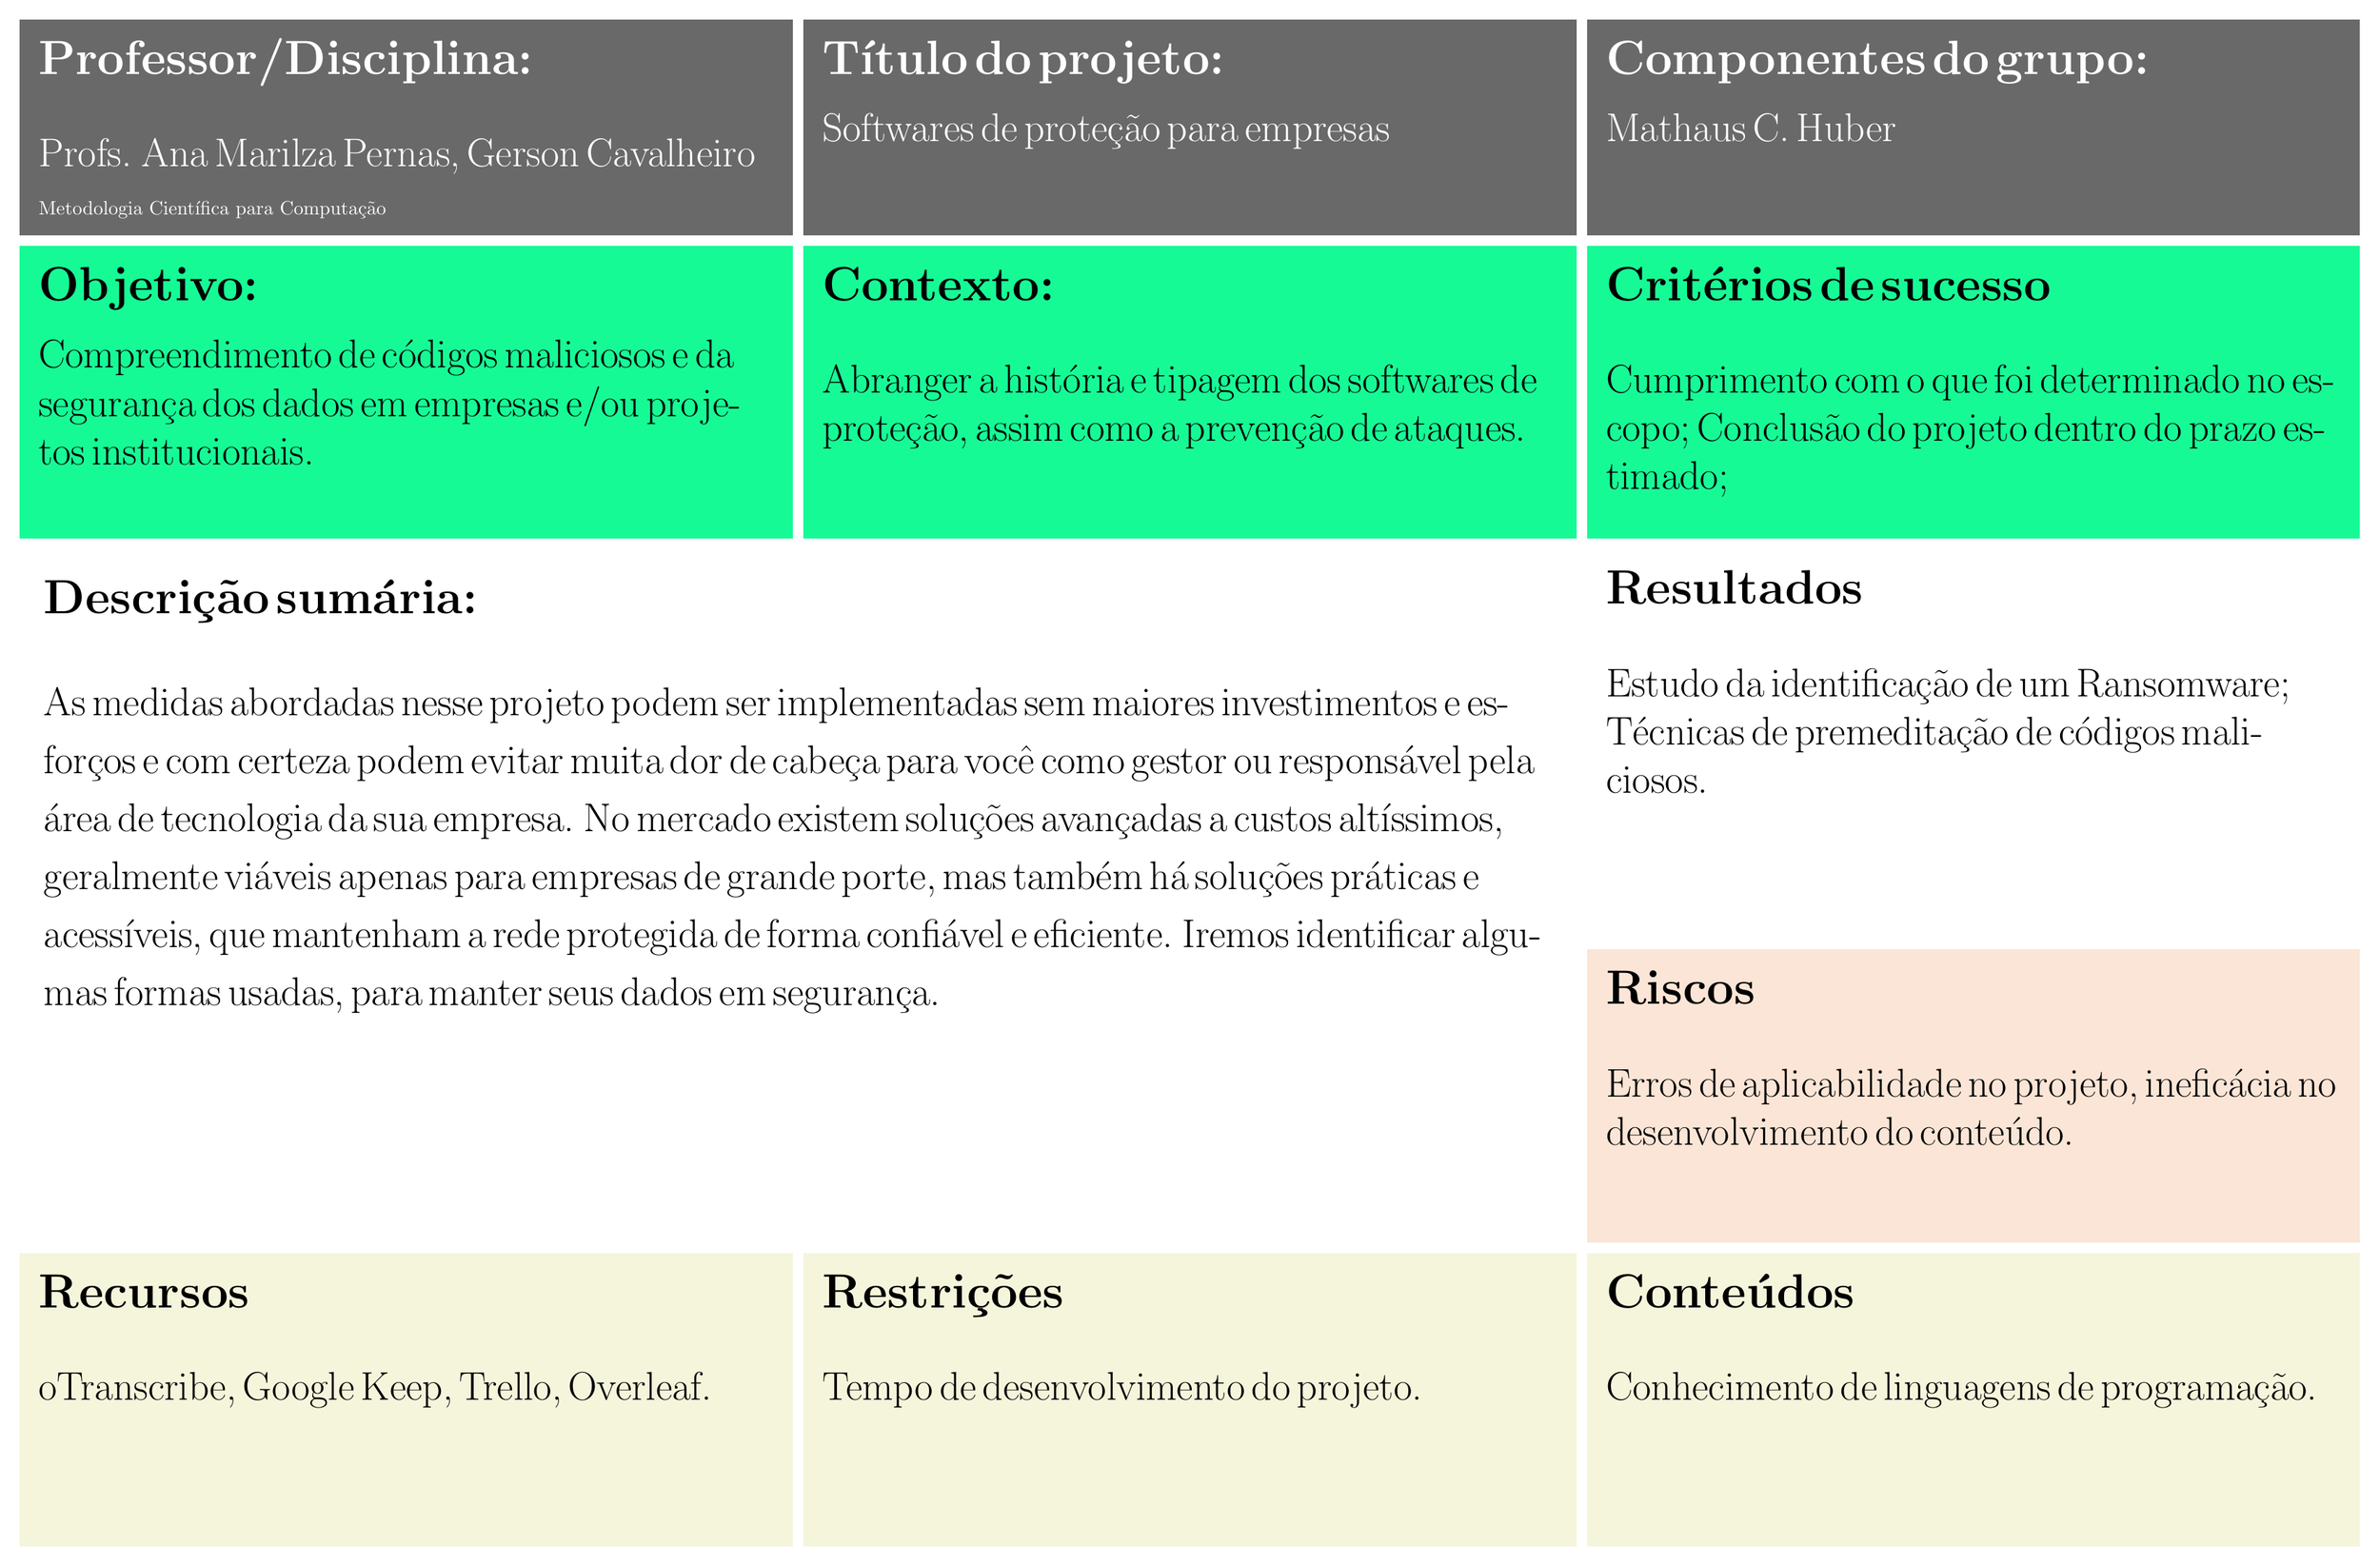
\begin{tikzpicture}

% Basic informationen
\client{Profs. Ana Marilza Pernas, Gerson Cavalheiro}{Metodologia Científica para Computação}
\project{Softwares de proteção para empresas} 
%\manager{Nome dos alunos} 
\developers{Mathaus C. Huber} 

% Project information
\why{Compreendimento de códigos maliciosos e da segurança dos dados em empresas e/ou projetos institucionais.}
\what{Abranger a história e tipagem dos softwares de proteção, assim como a prevenção de ataques.}
\success{Cumprimento com o que foi determinado no escopo; Conclusão do projeto dentro do prazo estimado;}
\outcome{Estudo da identificação de um Ransomware; Técnicas de premeditação de códigos maliciosos.}
    
% Project context
\risks{Erros de aplicabilidade no projeto, ineficácia no desenvolvimento do conteúdo. }

\stake{Conhecimento de linguagens de programação.}
\constraints{Tempo de desenvolvimento do projeto.}
\ressources{oTranscribe, Google Keep, Trello, Overleaf.}

% Project content
\content{As medidas abordadas nesse projeto podem ser implementadas sem maiores investimentos e esforços e com certeza podem evitar muita dor de cabeça para você como gestor ou responsável pela área de tecnologia da sua empresa.
No mercado existem soluções avançadas a custos altíssimos, geralmente viáveis apenas para empresas de grande porte, mas também há soluções práticas e acessíveis, que mantenham a rede protegida de forma confiável e eficiente.
Iremos identificar algumas formas usadas, para manter seus dados em segurança.}


\end{tikzpicture}
\end{document}